\documentclass[30pt,landscape,magscalefonts]{foils}
\usepackage{floatflt}
%\usepackage{times}
\usepackage{tabularx}
\usepackage[pdftex]{graphicx}
\graphicspath{{./graphics/}}
\usepackage[pdftex]{color}
\usepackage[pdftex]{geometry}
\geometry{headsep=2.0em,hscale=0.80}
\usepackage{hyperref}
\hypersetup{
  pdftitle={SDR 2003 Report on Player},
  pdfauthor={Brian P. Gerkey, USC Robotics Research Lab},
  pdfpagemode={FullScreen},
  pdfborder={0 0 0}
}
%\usepackage{background}

% define some nice colors
\definecolor{myred}{rgb}{0.6,0,0}
\definecolor{myblue}{rgb}{0,0.2,0.4}
% set default text color
\color{myblue}

% don't want any paragraph indentation
\setlength{\parindent}{0cm}

% wrapper for foilhead that sets the text color
\newcommand{\foilheadc}[1]{\foilhead{\Large \textcolor{myred}{#1}}\vspace*{-2em}}
% wrapper for itemize that shortens the inter-item separation
\newenvironment{xitemize}{\begin{itemize} \itemsep 1pt}{\end{itemize}}
% wrapper for enumerate that shortens the inter-item separation
\newenvironment{xenumerate}{\begin{enumerate} \itemsep 1pt}{\end{enumerate}}

\def\movieroot{file:///mnt/win/users/gerkey/videos}

\title{\textcolor{myred}
{\large The Player/Stage Project:\\ Tools for Multi-Robot and Distributed
Sensor Systems}}
\author{\small Brian P. Gerkey\hspace{1.5em} Richard T. Vaughan\hspace{1.5em}
Andrew Howard\vspace*{1em}\\

\includegraphics[height=15mm]{cres-logo.jpg}

\includegraphics[height=15mm]{usclogo.jpg}\hspace*{2em}

\includegraphics[height=15mm]{hrl_logo.jpg} \vspace*{1em}\\
{\tt \small http://playerstage.sourceforge.net}}
\date{}

% headers, etc.
\rightheader{

\includegraphics[height=15mm]{cres-logo.jpg}

\includegraphics[height=15mm]{usclogo.jpg}
}
\leftheader{
\includegraphics[height=15mm]{hrl_logo.jpg}}
\MyLogo{}
\def\totalpages{\pageref{lastpage}}
\rightfooter{\textcolor{myblue}{\quad\textsf{\thepage/\totalpages}}}

\begin{document}

% the title slide
\maketitle

% get the page numbering right
\pagebreak\setcounter{page}{2}

\foilheadc{The problem}
\begin{itemize}
\item Robotics is (largely) concerned with the synthesis of physical
sensor-actuator systems.
\item Interacting with these systems requires a significant amount of
infrastructure:
{\small
\begin{itemize}
\item a programmer's interface to robotic devices
\item a simulator
\end{itemize}
}
\item Multi-robot systems add complications:
{\small
\begin{itemize}
\item more robots
\item network programming
\end{itemize}
}
\end{itemize}

\foilheadc{The problem (cont'd)}
Good infrastructure for robotics research should be neutral with respect
to:
{\small
\begin{xitemize}
\item programming language
\item computing platform
\item control architecture
\item \fbox{robot hardware}
\item \fbox{physical location}
\end{xitemize}
}
It should also be {\bf Free}.

\foilheadc{Our solution}
The Player/Stage project is a collaborative development effort aimed at
producing high-quality Open Source tools for robotics researchers.

\vspace{1em}
The project primarily maintains two pieces of software:
\begin{itemize}
\item {\bf Player}: A networked robot device server.
\item {\bf Stage}: A multiple robot simulator.
\end{itemize}

\foilheadc{Player}
\MyLogo{Gerkey, et al., ``Most Valuable Player: A Robot Device Server for
Distributed Control,'' IROS 2001.}
Player is a socket-based device server, built on three key abstractions,
borrowed from operating systems design:

\begin{tabular}{cc}
\parbox{.6\textwidth}{
\begin{itemize}
\item {\tt read}/{\tt write}/{\tt ioctl}
\item interface/driver
\item client/server
\end{itemize}}
&
\parbox{.5\textwidth}{\hspace*{-4em}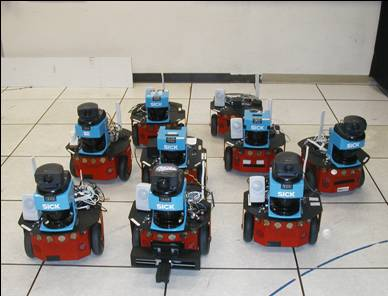
\includegraphics[width=.5\textwidth]{uscpioneers.jpg}}
\end{tabular}

\foilheadc{Stage}
\enlargethispage{2em}
\vspace*{-.7em}
\MyLogo{}
Stage is a highly configurable and scalable sensor-based multiple robot 
simulator.
\begin{xitemize}
\item All devices controlled through Player.
{\small
\begin{xitemize}
\item Many controllers have been shown to transfer between simulation and
hardware with {\bf no} changes.
\end{xitemize}
}
\item Robots move in 2D bitmapped world.
\item Models designed to scale to large populations.
{\small
\begin{itemize}
\item Computation scales linearly with population
\item User specifies world resolution.
\item Simulate 100s of robots w/ sonar, odometry, etc.
\item Simulate 10s of robots w/ laser, vision, etc.
\end{itemize}
}
\end{xitemize}

\foilheadc{An example world}
\begin{center}
\href{\movieroot/stage-everything.mpg}{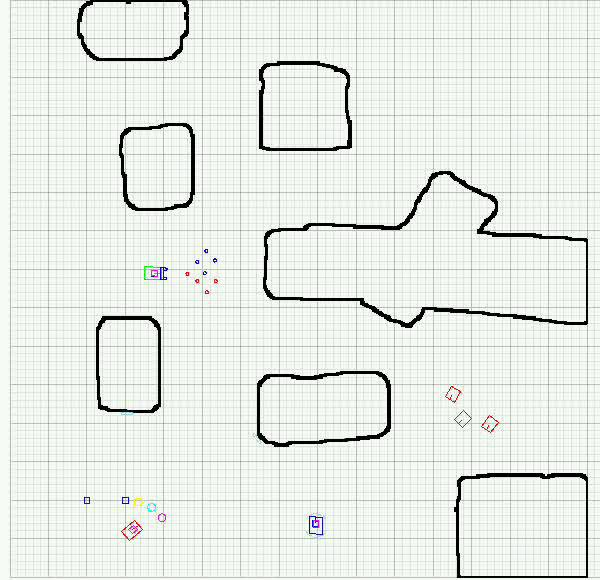
\includegraphics[height=130mm]{stage-everything.jpg}}
\end{center}

\foilheadc{Interfaces vs.\ drivers}
\MyLogo{Vaughan, et al., ``On device abstractions for portable, reusable 
robot code,'' IROS 2003.}
{\small
\begin{xitemize}
\item A device {\em interface}, such as {\bf position}, is a generic
specification of the format for data, command, and configuration
interactions.
\item A device {\em driver}, such as {\bf pioneer-position} or {\bf
rwi-position}, specifies how the low-level device control will be carried
out.
\item Multiple drivers (both real and simulation) can present the same 
interface.
\item The {\bf same} controller can be used with {\bf different} devices.
\end{xitemize}}

\foilheadc{Sophisticated drivers}
\MyLogo{}
{\small
\begin{itemize}
\item Drivers can do much more than provide transparent access to a device.
\item Arbitrary computation can be embedded in a driver.
\item Well-understood algorithms can be encapsulated in Player and
offered as standard services.
\item Examples: acoustic filtering, probabilistic localization,
obstacle avoidance.
\item Player becomes a community code repository.
\end{itemize}
}


\foilheadc{An example sophisticated driver}
The {\bf laser-visual fiducial-finder}:

\begin{tabular}{cc}
\parbox{.7\textwidth}{
\begin{itemize}
\item Uses laser range-finder, PTZ camera and color segmenter to locate and 
identify fiducials.
\item Performs sensor fusion on range and image data.
\item Includes closed-loop control of PTZ camera.
\end{itemize}}
&
\parbox{.3\textwidth}{\href{\movieroot/lvb.avi}{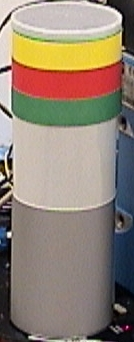
\includegraphics[width=.21\textwidth]{laservisualbeacon2.jpg}}}
\end{tabular}

\foilheadc{A very different kind of robot}
\vfill
\begin{center}
\href{\movieroot/rmp-wallfollow-1.5mps.avi}{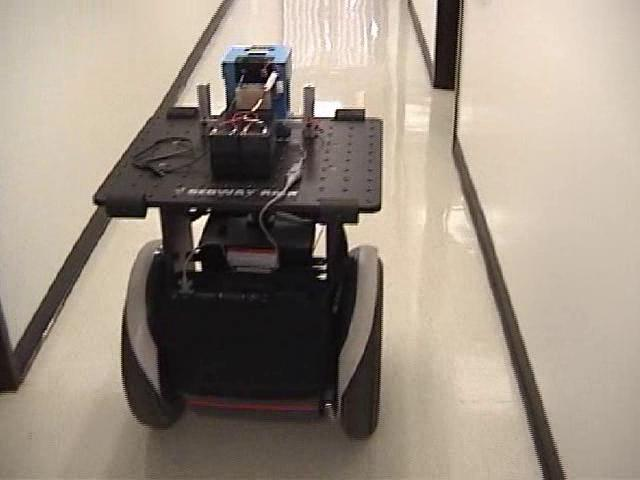
\includegraphics[width=.4\textwidth]{rmp-wallfollow-15mps.jpg}}
\href{\movieroot/rmp-outdoor-slalom.avi}{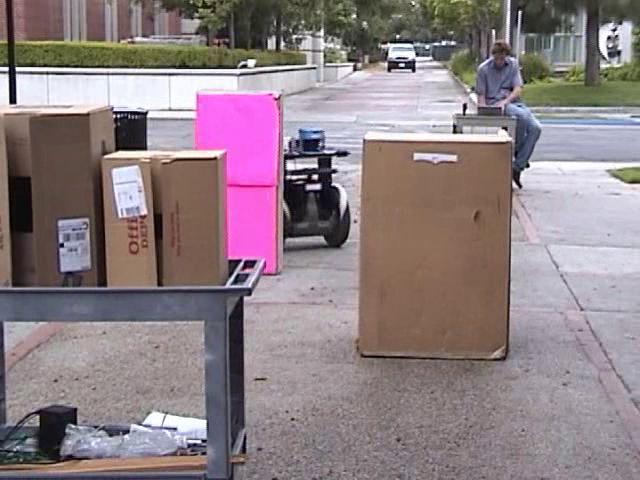
\includegraphics[width=.4\textwidth]{rmp-outdoor-slalom.jpg}}
\end{center}
\vfill

\foilheadc{Shifting the computation}
\begin{xitemize}
\item When an algorithm is implemented as a driver, the associated
computational load is moved to the server.
\item The {\bf passthrough} driver acts as a proxy within one server
for a device in another server.
\item Allows computational load to be shifted arbitrarily, within a
network or across the Internet.
\item Also allows one server to aggregate and distribute data and
commands for multiple robots.
\end{xitemize}

\foilheadc{Passthrough examples}
\vspace*{-.7em}
\rightfooter{}
\enlargethispage{5em}
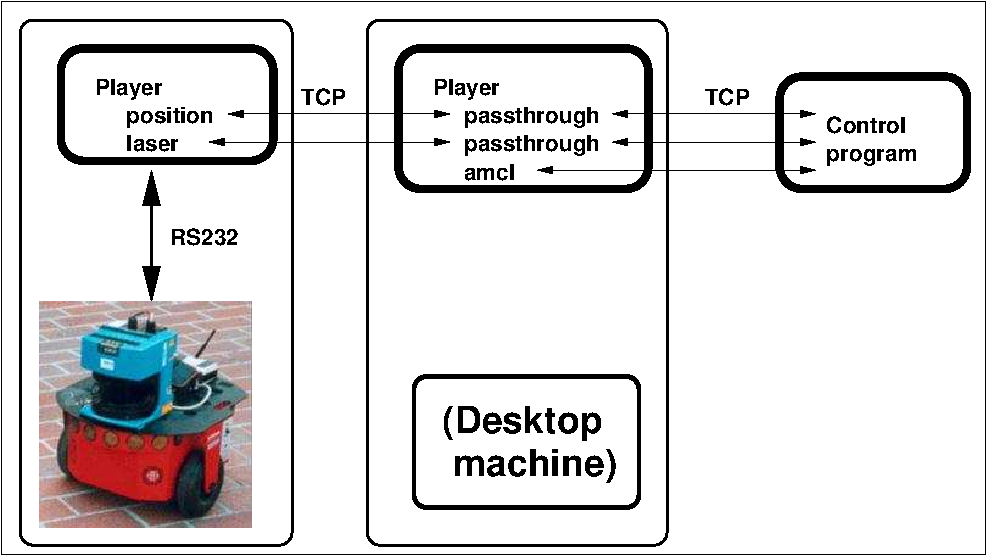
\includegraphics[width=0.7\textwidth]{passthrough1.pdf}

\hfill 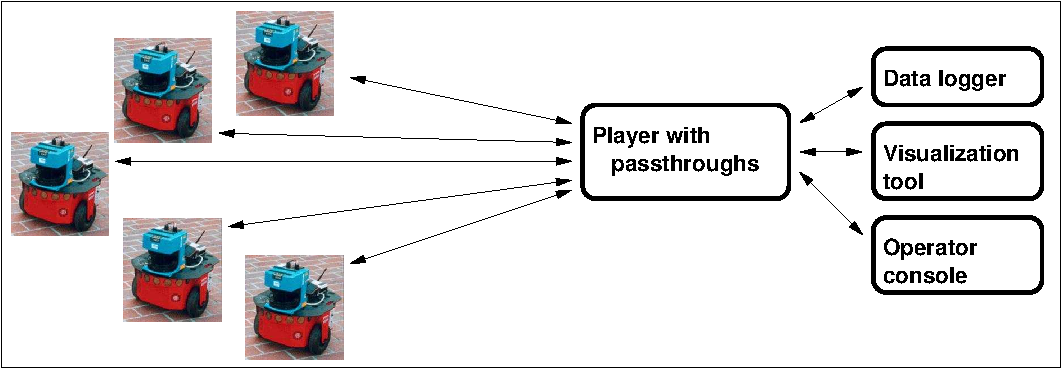
\includegraphics[width=0.8\textwidth]{passthrough2.pdf}

\foilheadc{Disruptive technology?}
\rightfooter{\textcolor{myblue}{\quad\textsf{\thepage/\totalpages}}}
{\small
\begin{xitemize}
\item Standard set of devices
\item Standard device abstractions
\item Standard transport (client$\leftrightarrow$device comms)
\item Standard sensor processing devices
\item Standard environments
\item Standard tasks
\item Standard metrics
\end{xitemize}
}

$\Rightarrow$ compare your control techniques with others

\foilheadc{Fantastic sensors}
While most Stage devices model real hardware, Stage can also be
used as a ``what if'' tool, e.g.:
{\small
\begin{itemize}
\item How would my localization algorithm perform with a device that
performs half-way between a sonar and a laser?
\item What are the trade-offs between robot speed and battery life,
or sensor update rates and resolution?
\item What novel algorithms could exploit an ultra-wide-band radar that
could detect walls {\it and} the objects behind them?
\end{itemize}
}

\foilheadc{Summary}
{\small
\begin{xitemize}
\item All Player/Stage software is Open Source (released under the GNU
GPL), and runs on most POSIX-like platforms.
\item Player supports (and Stage models) many common research robots and 
peripherals.
\item Player's network-centric design facilitates novel distributed sensing
and control systems.
\item Sophisticated sensing and control algorithms can be encapsulated as
Player drivers.
\item Stage is a tool for comparison and design of algorithms.
\end{xitemize}
}

\foilheadc{Acknowledgments}
\enlargethispage{5em}
{\tiny
{\bf Developers}:
Maxim Batalin,
Josh Bers,
Matt Brewer,
Brendan Burns,
Jason Douglas,
Jakob Fredslund,
Reed Hedges,
Kim Jinsuck,
Boyoon Jung,
Alex Makarenko,
Andy Martignoni III,
Nik Melchior,
Dave Naffin,
Esben \O{}sterg\aa{}rd,
Gabe Sibley,
Kasper St\o{}y,
John Sweeney,
Doug Vail.\\
{\bf Support}:
Maja Matari\'{c} \& Gaurav Sukhatme @ USC, Dave Payton @ HRL\\
{\bf Project management}: SourceForge.net
}
\begin{center}
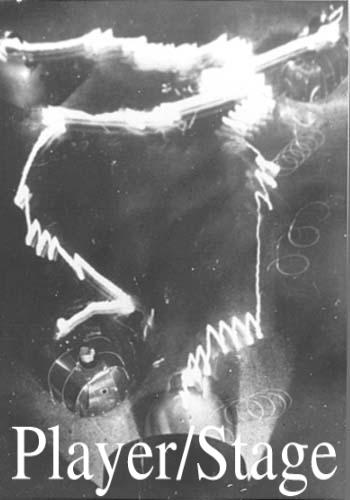
\includegraphics[height=60mm]{ps_logo.jpg}\\
\fbox{\small \tt http://playerstage.sourceforge.net}
\end{center}

\foilheadc{Another movie}
\vfill
\begin{center}
\href{\movieroot/rmp-fall.avi}{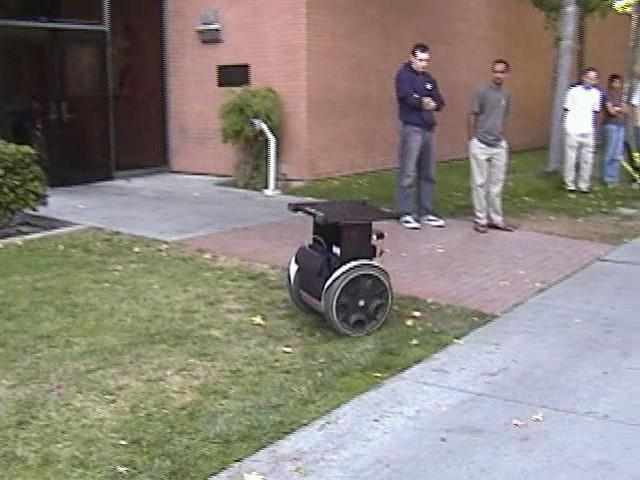
\includegraphics[width=.8\textwidth]{rmp-fall.jpg}}
\end{center}
\vfill

\foilheadc{Yet another movie}
\label{lastpage}
\vfill
\begin{center}
\href{\movieroot/stage-table.mpg}{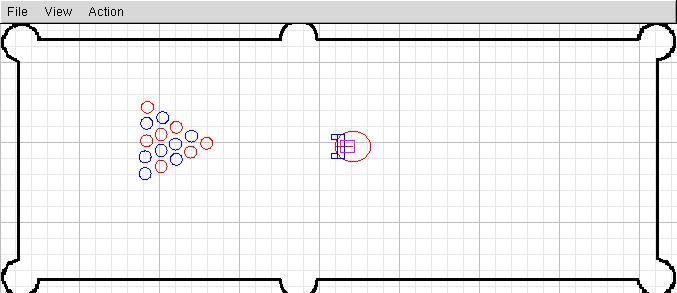
\includegraphics[width=\textwidth]{stage-table.jpg}}
\end{center}
\vfill

\end{document}
